% \chapter{Marco Te\'orico}

% \section{Modelo relacional}

% \begin{definition}
%     Una \textbf{relaci\'on} $R$ sobre un conjunto de dominios $D_1, D_2, ..., D_n$,
%     (no necesariamente todos distintos) se compone de dos partes:
%     una cabecera y un cuerpo, donde:
%     \begin{itemize}
%         \item La \textbf{cabecera} est\'a formada por un conjunto finito de
%         pares atributo-dominio $\{(A_1, D_1), (A_2, D_2), ..., (A_n, D_n)\}$,
%         tal que a cada atributo $A_j$ corresponde a uno y solo uno de los dominios
%         subyacentes $D_j, (j=1,2,...,n)$.
%         \item El \textbf{cuerpo} est\'a formado por un conjunto finito de tuplas, el cual
%         var\'ia en el tiempo. Cada tupla, a su vez, est\'a formada por un conjunto
%         de pares atributo-valor, $\{(A_1, V_{i1}), (A_2, V_{i2}), ..., (A_n, V_{in}) \}, (i = 1,2,...,m)$
%         tal que $m$ es el n\'umero de tuplas en el conjunto tal que, para cada
%         par $(A_j, V_{ij}),\; V_{ij}$ es un valor del dominio $D_j$ asociado al atributo
%         $A_j, (j=1,2,...,n)$ 
%     \end{itemize}
% \end{definition}

% \section{Teor\'ia de Grafos}

% Los grafos son estructuras de datos utilizadas extensivamente
% dentro de la Ciencia de la Computaci\'on. Debido a su capacidad
% para representar la existencia de relaciones entre elementos han sido empleados para
% modelar fen\'omenos tan diversos como las redes sociales, estructuras moleculares,
% interacciones biol\'ogicas entre prote\'inas, preferencias de usuarios, entre muchos otros.

% \subsection{Tipos de Grafos}


% \subsection{Graph Embedding}

% \begin{definition}
%     Dado un grafo $G = (V,E)$ una \textbf{medida de similaridad} sobre el
%     conjunto de v\'ertices $V$ es una funci\'on $f : V \times V \to \mathbb{R}$ 
%     la cual indica la similaridad entre dos v\'ertices del grafo.
% \end{definition}

% \begin{definition}
%     El \textbf{problema de graph embedding} consiste en dado un grafo
%     $G = (V,E)$ y un entero $k$, tal que $k \ll |V|$, representar el
%     grafo $G$ en un espacio $k$-dimensional en el cual se deben de preservar
%     las propiedades de dicho grafo. Estas propiedades pueden ser
%     especificadas mediante la definici\'on de medidas de similaridad.
% \end{definition}

% En \textit{graph embedding} un grafo puede ser representado como un
% vector de $k$ dimensiones o como un conjunto de vectores de $k$ dimensiones
% los cuales representan alg\'un componente del grafo (v\'ertices, aristas o subestructuras).
% % \begin{definition}
% %     Sea un grafo $G = (V,E)$ la \textbf{proximidad de primer orden} $s_{ij}^{(1)}$ entre los v\'ertices $v_i$ y $v_j$
% %     es el peso de la arista $e_{ij}$. Se denota $s_i^{(1)} = [s_{i1}^{(1)}, s_{i2}^{(1)},..., s_{i|V|}^{(1)} ]$ a la proximidad
% %     del v\'ertice $v_i$ con el resto del grafo.
% % \end{definition}

% % \begin{definition}
% %     Sea un grafo $G = (V,E)$ la \textbf{proximidad de segundo orden} $s_{ij}^{(2)}$ entre los v\'ertices $v_i$ 
% % \end{definition}

% \subsection{Graph Embeddings}

% \begin{definition}
    
% \end{definition}







\chapter{Estado del Arte}\label{chapter:state-of-the-art}

\section{Lenguajes de Visualizaci\'on de Datos}
Los lenguajes de visualizaci\'on de datos son utilizados para especificar
relaciones entre los datos a visualizar y los componentes gr\'aficos.

La mayor\'ia de lenguajes de visualizaci\'on se enfocan en brindar a los usuarios humanos
un marco para definir los datos de inter\'es y c\'omo deben ser visualizados [\cite*{li2018echarts}, \cite*{tableau}]. 
Estos est\'an compuestos por datos (registros y transformaciones), 
componentes gr\'aficos (marcas, leyendas, ejes, etc...) y
m\'etodos para definir una funci\'on de correspondencia entre ambos. Suelen clasificarse
de acuerdo a su expresividad en lenguajes de bajo nivel y lenguajes de alto nivel \cite{qin2020making}.

Otros sistemas se enfocaron en dar una definici\'on m\'as conveniente de procesar
por algoritmos basados en inteligencia artificial permitiendo definir espacios de b\'usqueda de
visualizaciones \cite{godfrey2016interactive}.


\subsection{Lenguajes de Visualizaci\'on de Datos de Bajo Nivel}
Los lenguajes de bajo nivel son aquellos en los que el usuario debe de especificar c\'omo asociar los
datos a cada componentes gr\'afico utilizado, permitiendo un alto nivel de personalizaci\'on y detalle en
las visualizaciones resultantes.

Los lenguajes de prop\'osito general pueden utilizarse como lenguaje de visualizaci\'on de bajo nivel
mediante la implementaci\'on de bibliotecas de visualizaci\'on. Algunas de las bibliotecas desarrolladas
con este prop\'osito han sido Prefuse \cite{heer2005prefuse} en Java y Matplotlib \cite{matplotlib} en Python,
estos lenguajes orientados a objetos modelan
los elementos gr\'aficos mediante clases las cuales implementan m\'etodos para definir el mapeo con los datos.

Otra alternativa ha sido el desarrollo de lenguajes
de dominio espec\'ifico (DSL por sus siglas en ingl\'es) dentro de lenguajes de alto nivel. Por ejemplo,
Protovis \cite{bostock2009protovis} es un DSL desarrollado en JavaScript 
el cual est\'a enfocado en brindar las mayores capacidades de personalizaci\'on para el usuario.

Varios de estos lenguajes han sido dise\~nados con el fin de ser un lenguaje independiente utilizado como est\'andar
de especificaci\'on de visualiaciones para permitir su uso entre varias plataformas. Este es el caso de
Vega \cite{vegaLang} y ReactiveVega \cite{satyanarayan2015reactive} los cuales permiten definir visualizaciones utilizando
un paradigma declarativo sin estar contenidos dentro de otro lenguaje y han sido utilizados por varias plataformas de
visualizaci\'on.

\subsection{Lenguajes de Visualizaci\'on de Datos de Alto Nivel}
Los lenguajes de alto nivel permiten abstraer al usuario de ciertos elementos dentro de la construcci\'on
de las visualizaciones mediante la utilizaci\'on de valores por defecto y la adici\'on de restricciones a sus capacidades. Estos pueden
estar implementados sobre lenguajes de bajo nivel y suelen ser m\'as f\'aciles de utilizar por los usuarios.
%[Figura \ref{fig: vega_vs_vega_lite}].

Muchos de estos lenguajes han surgido durante el desarrollo de plataformas
de an\'alisis de datos enfocadas a usuarios sin conocimientos en programaci\'on para mejorar la experiencia de uso. 
Plataformas como Echarts con lenguaje de nombre hom\'onimo \cite{li2018echarts} y Tableau la cual utiliza VizQL \cite{hanrahan2006vizql}
permiten a los usuarios especificar visualizaciones con una sintaxis simple y concisa.

Otros lenguajes han sido dise\~nados para facilitar el desarrollo de ecosistemas de
visualizaci\'on de datos en torno a ellos. Por ejemplo, Vega-Lite \cite{satyanarayan2016vega} es un lenguaje actualmente utilizado
por m\'ultiples plataformas de an\'alisis de datos y ha sido llevado a lenguajes como Python, Ruby y R mediante
la implementaci\'on de bibliotecas como Altair, Vega.rb y Elm-Vega respectivamente \cite{vegaEco}.

Igualmente se pueden econtrar implementaciones dentro de otros lenguajes como gg2plot implementado
directamente sobre el lenguaje R \cite{wickham2010layered}.

\subsection{Lenguajes basados en predicados l\'ogicos}

Los lenguajes de visualizaci\'on basados en predicados l\'ogicos surgen
con las primeras aproximaciones de los cient\'ificos al problema de visualizaci\'on autom\'atica de
datos. Estos lenguajes han sido utilizados para modelar los espacios de b\'usqueda que utilizan los algoritmos
enfocados a resolver este problema \cite{godfrey2016interactive}.

Este tipo de enfoques intentan representar el conocimiento humano existente \cite{bertin1983semiology} en el dise\~no
de visualizaciones a trav\'es de definir condiciones l\'ogicas las cuales pueden ser comprobadas de forma
secuencial mediante instrucciones \textit{if-then-else} [\cite*{mackinlay1986automating}, \cite*{mackinlay2007show}, \cite*{roth1994interactive}, \cite*{wongsuphasawat2015voyager}, \cite*{moritz2018draco}].


% \begin{figure}[h!]
%     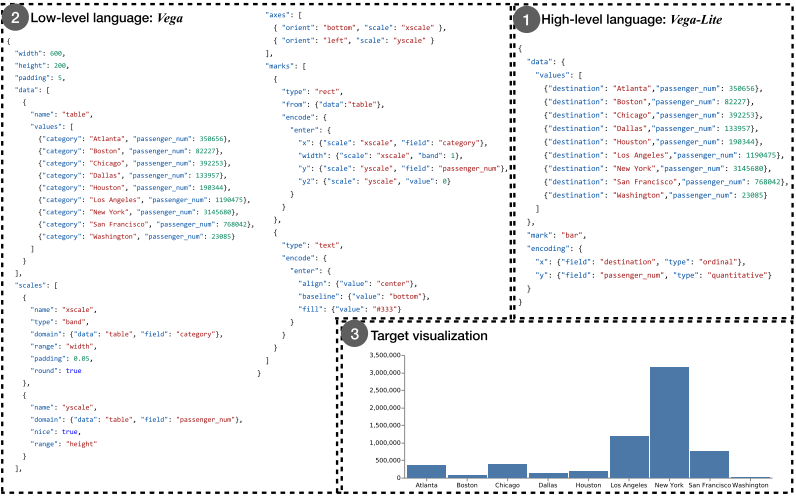
\includegraphics[width=\linewidth, height=70mm]{Graphics/vega_vs_vega_lite.png}
%     \caption{Comparaci\'on de complejidad entre los lenguajes Vega y Vega-Lite. 
%      (1) Ejemplo de c\'odigo utilizando el lenguaje Vega, (2) ejemplo de c\'odigo utilizando el lenguaje Vega-Lite,
%      (3) visualizaci\'on resultante en ambos casos.}
%     \label{fig: vega_vs_vega_lite}
% \end{figure}


\section{Sistemas de Recomendaci\'on de Visualizaciones}

La visualizaci\'on inteligente autom\'atica de datos tiene como objetivo
principal reducir el tiempo y esfuerzo necesitado para la exploraci\'on y
an\'alisis visual de los conjuntos de datos \cite{zeng2021we}. 

Las propuestas para
resolver dicho problema son denominados sistemas de recomendaci\'on de
visualizaciones (VizRec) y son un mecanismo de b\'usqueda en el espacio de visualizaciones
de acuerdo al inter\'es personalizado del usuario. A pesar de que el t\'ermino
VizRec fue recientemente concebido \cite{vartak2017towards}, el \'area, como tal, no es nueva.
Los primeros sistemas en generar visualizaciones de forma autom\'atica aparecer\'ian
a partir del a\~no 1986, manteniendose un alto inter\'es en el campo con el desarrollo
de nuevas soluciones y sistemas hasta la actualidad \cite{godfrey2016interactive}. 

Generalmente estos sistemas funcionan siguiendo un mismo procedimiento de dos pasos:
\begin{enumerate}
    \item Enumerar un conjunto de visualizaciones de inter\'es a partir de un espacio de visualizaciones.
    \item Utilizar una funci\'on de \textit{ranking} para ordenar el conjunto resultante.
\end{enumerate}

Actualmente existen dos enfoques principales para implementar este proceso: el enfoque basado en reglas
y el enfoque basado en aprendizaje de m\'aquinas. Los primeros han sido altamente estudiados dentro de la 
literatura debido que los primeros sistemas en aparecer fueron basados en reglas y la existencia
de numerosos trabajos acerca de pr\'acticas y heur\'isticas para dise\~no de visualizaciones facilitaba su desarrollo.
Por otro lado los enfoques basados en aprendizaje de m\'aquinas han tomado relevancia en los \'ultimos a\~nos con la aparici\'on
de varios prototipos \cite{zeng2021we}.

\subsection{Recomendaci\'on de Visualizaciones Basada en Reglas} \label{subsection:rule-viz-rec}

Los sistemas de recomendaci\'on basados en reglas se caracterizan por el establecimiento
de condiciones bien definidas para la recomendaci\'on de visualizaciones. Estos sistemas
se pueden diferenciar de acuerdo al marco sobre el que se definen las condiciones: unos sistemas
se enfocan en representar el conocimiento humano en visualizaci\'on mediante programaci\'on l\'ogica y 
otros se centran en la utilizaci\'on de m\'etricas para la comparaci\'on de visualizaciones.

Los primeros sistemas en aparecer fueron basados en programaci\'on l\'ogica, estos propon\'ian lenguajes
l\'ogicos especiales para la representaci\'on de visualizaciones mediante un conjunto de reglas las cuales
se pod\'ian comprobar mediante instrucciones condicionales.

\textbf{Automatic Presentation Tool} (APT) \cite{mackinlay1986automating} fue el primer sistema de recomendaci\'on de visualizaciones.
En este enfoque las visualizaciones son definidas como oraciones de lenguajes
de visualizaci\'on de datos. Las consideraciones asociadas al dise\~no de visualizaciones
fueron implementadas como criterios de comparaci\'on para estos lenguajes. El criterio de expresividad
evaluaba cu\'anta informaci\'on (patrones, tendencias, anomal\'ias, etc...) era capaz de
transmitir el lenguaje. El criterio de efectividad evaluaba la utilizaci\'on de los
elementos gr\'aficos para facilitar la comprensi\'on de la informaci\'on transmitida.
El sistema generaba dise\~nos de forma autom\'atica utilizando composiciones algebraicas
de lenguajes de visualizaci\'on primitivos, luego los dise\~nos obtenidos eran recomendados de acuerdo
a los criterios de expresividad y efectividad.


\textbf{SAGE} \cite{roth1994interactive} extendi\'o la soluci\'on propuesta por APT al permitir
la especificaci\'on total o parcial de las visualizaciones por los usuarios. Estas especificaciones
eran tratadas como directrices de dise\~no las cuales restring\'ian el espacio de b\'usqueda
analizado por el algoritmo que construye y compara las visualizaciones. El sistema pod\'ia construir
visualizaciones a partir de especificaciones sobre la informaci\'on relevante a mostrar o sobre
elementos de dise\~no gr\'afico.


\textbf{Draco} \cite{saket2018beyond} est\'a enfocado en el paradigma de la programaci\'on
basada en restricciones dentro de la programaci\'on declarativa. Un programa de restricciones 
es un conjunto de restricciones las cuales definen las relaciones entre un conjunto de variables cuyo
valor es desconocido. Este sistema introduce dos tipos de restricciones: las restricciones fuertes
las cuales deben de ser cumplidas por las soluciones del problema y las restricciones d\'ebiles las cuales
pueden violarse al costo de dicha soluci\'on sea penalizada. Estas restricciones restringen los posibles
valores de las variables y modelan la informaci\'on parcial sobre dichas inc\'ognitas. Las soluciones son
computadas como las de un problema de optimizaci\'on combinatoria sujeto a restricciones. Draco implementa
esta idea mediante una representaci\'on l\'ogica del lenguaje de visualizaci\'on Vega-Lite sobre la
cual un conjunto de expertos definen las restricciones y los pesos en caso de ser restricciones suaves.

Los sistemas basados en m\'etricas se enfocan en utilizar medidas que caractericen la cantidad
de informaci\'on que transmite la visualizaci\'on. Estas m\'etricas provienen de distintas ramas
de la Matem\'atica y Computaci\'on. como .

Seo y col. \cite{seo2004rank} propone un sistema el cual recibe como especificaci\'on parcial el tipo de
gr\'afico (gr\'afico de barras, gr\'afico de puntos e histogramas), construye todos los posibles
gr\'aficos del tipo seleccionada y luego realiza un \textit{ranking} de acuerdo al valor de una m\'etrica seleccionada las
cuales eran espec\'ificas para cada tipo de gr\'afico. Por ejemplo, los histogramas utilizan m\'etricas enfocadas en propiedades
de la distribuci\'on de los datos mientras los gr\'aficos de puntos utilizaban la correlaci\'on, clusterizaci\'on y regresi\'on.

\textbf{SeeDB} \cite{vartak2014seedb} es un sistema el cual intenta maximizar el inter\'es del usario
al utilizar como referencia visualizaciones generadas o seleccionadas por el usuario
para recomendar aquellas visualizaciones que maximicen la desviaci\'on con los datos de la muestra.


\textbf{Foresight} \cite{demiralp2017foresight} realiza una clasificaci\'on de los tipos de gr\'aficos de
acuerdo al tipo de informaci\'on que pueden transmitir de acuerdo a consideraciones de dise\~no extra\'idas
de la literatura. Por ejemplo, los gr\'aficos de l\'inea suelen ser utilizados para mostrar correalaciones
mientras las gr\'aficas de caja permiten mostrar valores extremos. Esta clasificaci\'on permite reducir el tama\~no
del espacio de posibles visualizaciones mejorando la eficiencia del sistema con respecto a \cite{seo2004rank}.
Adem\'as incorpora cierta retroalimentaci\'on por
parte del usuario recomendando aquellos gr\'aficos que muestren el mismo tipo de informaci\'on que el gr\'afico
seleccionado por el usuario. Posteriormente \textbf{SpotLight} \cite{harris2021insight} extender\'ia este trabajo soportando
m\'as tipos de gr\'aficos y utilizando variadas m\'etricas de la Estad\'istica, Teor\'ia de la informaci\'on e Inteligencia artificial.

Este tipo de enfoque suele tener graves problemas de eficiencia debido a que se realizan exploraciones exhaustivas de los
espacios de b\'usqueda por lo que \cite{vartak2014seedb} propuso varias estrategias como podas, computaci\'on distribuida, etc...
Por otra parte los sistemas basados en reglas han presentado problemas para realizar la comparaci\'on entre visualizaciones debido
a la dificultad de realizar una definici\'on l\'ogica de criterios los cuales pueden ser subjetivos \cite{vartak2017towards}.

\textbf{DIVE} \cite{hu2018dive} propone un enfoque h\'ibrido que intenta resolver estos problemas combinando
la generaci\'on de visualizaciones mediante la composici\'on de lenguajes con el \textit{ranking} basado en m\'etricas. 

\subsection{Recomendaci\'on de Visualizaciones Basada en Aprendizaje de M\'aquinas}\label{subsection:ml-viz-rec}
En la actualidad existen gran inter\'es en este tipo de enfoque apareciendo varias implementaciones
de estos sistemas con novedosas modelaciones del problema. 

\textbf{DeepEye} \cite{luo2018deepeye} divide el problema en dos subproblemas. El primer subproblema es modelado
como un problema de clasificaci\'on binaria donde utilizando \'arboles de decisi\'on se aprende a etiquetar 
como \textit{buenas} o \textit{malas} las visualizaciones generadas para un conjunto de datos. 
El segundo subproblema consiste en un problema de \textit{Learning to Rank} (LTR) sobre el conjunto de visualizaciones. 
Para resolver este problema se cre\'o un corpus con pares de visualizaciones y el resultado de su comparaci\'on, luego esta funci\'on fue aproximada
mediante el algoritmo RankNet \cite{luo2018deepeye}. Para realizar las recomendaciones el sistema genera todas las posibles visualizaciones y enumera
aquellas clasificadas como \textit{buenas} por el primer modelo, finalmente este conjunto es ordenado de acuerdo a la funci\'on de \textit{ranking} aprendidad por
el segundo modelo. 

\textbf{Draco-Learn} \cite{moritz2018draco} es una extensi\'on de la propuesta del sistema Draco discutido en la
secci\'on \ref{subsection:rule-viz-rec}, una de las limitaciones principales de este sistema era la necesidad
de que expertos del dominio ajustaran los pesos de las restricciones suaves de forma manual. Este nuevo sistema
utiliza RankSVM para ajustar de forma autom\'atica los pesos de las restricciones utilizando un corpus de visualizaciones
generadas por expertos.


\textbf{Data2Vis} \cite{dibia2019data2vis} transforma la recomendaci\'on de visualizaciones en un problema de
traducci\'on de lenguajes. Este sistema representa los datos de entrada mediante tuplas
relacionales definidas en el lenguaje JSON y su salida es un conjunto de sentencias
en el lenguaje de visualizaci\'on de datos Vega-Lite las cuales se corresponde con las
visualizaciones recomendadas. Esta traducci\'on se llev\'o a cabo utilizando m\'etodos
basados en redes neuronales recurrentes convencionales (RNN por sus siglas en ingl\'es).
Este tipo de redes neuronales son capaces de capturar el contexto de las oraciones debido
a sus estructuras de memoria y son muy utilizadas en sistemas de traducci\'on autom\'atica \cite{sutskever2014sequence}.


Quian y col. \cite{qian2020ml} propusieron un sistema basados en redes neuronales profundas. Este trabajo modela
la recomendaci\'on autom\'atica como un conjunto de problemas de clasificaci\'on multiclase sobre las configuraciones gr\'aficas
presentes en un lenguaje de visualizaci\'on. Por cada
configuraci\'on gr\'afica construyen un modelo que clasifica dicha configuraci\'on en sus respectivas opciones, por ejemplo,
la configuraci\'on \textit{eje} puede ser clasificada en \textit{x} o \textit{y}. De esta forma el sistema puede
seleccionar las opciones y construir las visualizaciones.


\section{Recomendaci\'on de Configuraciones Visuales}

Debido a la complejidad del problema de recomendaci\'on de visualizaciones muchos
sistemas optaron por intentar resolver un subproblema del mismo,
asumiendo la existencia de una especificaci\'on parcial de la visualizaci\'on donde el usuario haya seleccionado
los datos de inter\'es a visualizar. Esta versi\'on simplificada se plantea como el problema de la
recomendaci\'on autom\'atica de configuraciones gr\'aficas \cite{qin2020making}.

Siendo un subproblema del problema de recomendaci\'on de visualizaciones al igual que en este las implementaciones
de estos sistemas son basadas en reglas o basadas en aprendizaje de m\'quinas.

% BOZ \cite{casner1991task} recib\'ia como entrada una descripci\'on l\'ogica de
% una tarea de an\'alisis a realizar sobre el conjunto de datos, esta descripci\'on estaba
% basada en operadores l\'ogicos (representan operaciones sobre los datos) los cuales eran
% sustuidos por operadores perceptuales (representan el uso de componentes gr\'aficos) mediante
% el cumplimiento de reglas \textit{if-then-else}.
\subsection{Recomendaci\'on de Configuraciones Visuales Basada en Reglas}

Este tipo de sistemas basados en reglas son los utilizados actualmente por varias plataformas
de an\'alisis de datos.

\textbf{ShowMe} \cite{mackinlay2007show} es un sistema basado en APT cuyo enfoque fue expuesto en la secci\'on \ref{subsection:rule-viz-rec}. Este
trabajo introdujo el lenguaje de visualizaci\'on de datos de alto nivel llamado VizQL \cite{hanrahan2006vizql} el cual permite
especificar de forma algebraica la estructura de los gr\'aficos y los datos utilizados para generarlo.
Este sistema est\'a enfocado en la presentaci\'on visual y la experiencia de usuario por lo que las reglas y heur\'isticas implementadas
est\'an altamente influenciadas por los trabajos sobre dise\~no de visualizaciones y las m\'etricas utilizadas tienen como objetivo la expresividad de las visualizaciones. 

Por otro lado \textbf{Voyager} \cite{wongsuphasawat2015voyager} se enfoca en recomendar visualizaciones que muestren transformaciones sobre los datos seleccionados mediante
la utilizaci\'on de m\'etricas. Las configuraciones visuales son seleccionadas mediante la aplicaci\'on de reglas y heur\'isticas basadas en la literatura.   

\subsection{Recomendaci\'on de Configuraciones Visuales Basada en Aprendizaje de M\'aquinas}

Esta \'area ha comenzado a ser explorada recientemente con el desarrollo de \textbf{VizML} \cite{hu2019vizml}. Este sistema es el predecesor
del enfoque propuesto por Quin y col. en la secci\'on \ref{subsection:ml-viz-rec} y modela este problema como una serie de problemas de
clasificaci\'on multiclase sobre las configuraciones gr\'aficas de un lenguaje de visualizaci\'on. \textbf{KG4Vis} \cite{li2021kg4vis} utilizando
como referencia el trabajo realizado en VizML desarroll\'o un sistema donde la selecci\'on de las configuraciones gr\'aficas en el lenguaje se realiza
mediante la soluci\'on de problemas de \textit{link prediction} en un grafo de conocimientos.








